%!TEX root = ../master_thesis.tex

\section{Software environment terminology}
\label{sec:software_environment_terminology}

In this chapter we propose our software environment terminology model describing the microservice architectural style. We present the individual terms and the connections between them, and reflect on some related work. Extending the architectural model, we also introduce related infrastructural systems, which are commonly utilized when realizing such an architecture.

\subsection{The microservice architectural style}

Our terminology model is similar to the field of ``Service-oriented architecture'' (short: \emph{SOA}) (e.g. described by Krafzig in \cite{enterpriseSOA} and standardized by OASIS in \cite{oasissoa}). We did not find the SOA model to be a fitting description for the microservice architectural style, which is why we propose our own model here. This chapter is not an exhaustive survey over the usage of the introduced terms, but rather sets the stage for the remainder of our work.

\subsubsection{Software architecture}

To define \emph{software architecture}, we follow the model from Fielding~\cite{Fielding}:

``A software architecture is an abstraction of the run-time elements of a software system during some phase of its operation''~\cite{Fielding}. Run-time elements are usually separated into components and connections. Since a \emph{software architecture} is an abstraction, the exact definition of what constitutes a component and a connection depends on the level of detail and purpose of the current view on the software system. For example in this work we will often use applications as the granularity level for components and application dependencies as the granularity level for connections.

``A system may be composed of many levels of abstraction and many phases of operation, each with its own software architecture''~\cite{Fielding}. The different levels manifest themselves most prominently in the fact that each component in an architecture may consist of another architecture in itself. Continuing with the example from above, one application might in itself have an architecture consisting of its deployed services, or how its internal code modules relate to each other. The phases of operation may be seen as changing over time (for example the architecture changed between an hour ago and now) or states (for example the architecture changed when a new application was introduced).

\subsubsection{Software architecture style}

\emph{Software architecture styles} try to categorize common aspects of \emph{software architectures}. These aspects might be similar patterns in structural organization, the same granularity of components and connectors or similar constraints on how these work together as one system \cite{Shaw1996} \cite{fowler-microservices}.

\subsubsection{Software as a Service}

\emph{Software as a Service} (SaaS) is a software delivery model, in which the software code, computing resources and user data are managed by a provider. The software is remotely accessed by the consumer via a thin client, most commonly a web browser \cite{Carraro}.

Traditional software delivery models involved shipping executable software to the users, who then operated them on their own computing resources \cite{swebok}. Since SaaS software is operated by the vendor, it is possible to release software at a higher rate, sometimes several times in a day \cite{etsydeploy} \cite{ContinuousDelivery}.

In this work, we are concerned with multi-user SaaS, thus all users use the same computing resources supplied by the vendor, they have the same service level agreements and limited customization options \cite{salesforce} \cite{Mietzner2009} \cite{Azeez2010}. One promising architectural style for building a multi-user SaaS is the \emph{microservice architecture style}, which we will introduce next.

% The following definition is given in \cite{zhangsaas}: ``[...] the SaaS delivery model essentially separates software ownership from the user—the owner is a vendor who hosts the software and lets the user execute it on-demand through some form of client-side architecture via the Internet or an intranet. This new model delivers software as utility services and charges on a per-use basis [...]''

% In  the authors define SaaS as ``software deployed as a hosted service and accessed over the Internet" and further define it technically as ``the SaaS provider hosts the application and data centrally—deploying patches and upgrades to the application transparently, and delivering access to end users over the Internet through a browser or smart-client application''.

\subsubsection{Microservice architectural style}
\label{subsec:microservice_architecture}

% \definition{A services architecture is a software architecture style consisting of applications that interact with each other through services.}

Fowler et al \cite{fowler-microservices} define the \emph{microservice architecture style} as ``an approach to developing a single application as a suite of small services, each running in its own process and communicating with lightweight mechanisms, often an HTTP resource API''. In our case, the ``single application'' is the \emph{SaaS} as experienced by the user.

\emph{Microservice architecture} shares concepts with the ``Service-oriented architecture'' (SOA) style, but we decided to not use the term SOA directly due to the ambiguity of its meaning (as described by Fowler et al \cite{FowlerSOAAmbiguity} and Partridge et al \cite{modServicesAnalysis}).

The terms following next are all to be seen in the context of microservice architecture, and therefore define it further.

\subsubsection{Application}
\label{ss:application}

\begin{figure}[h!]
  \caption{Entity-relationship model of the terms defined in this chapter}
  \label{fig:software-env-erm}
  \makebox[\textwidth][c]{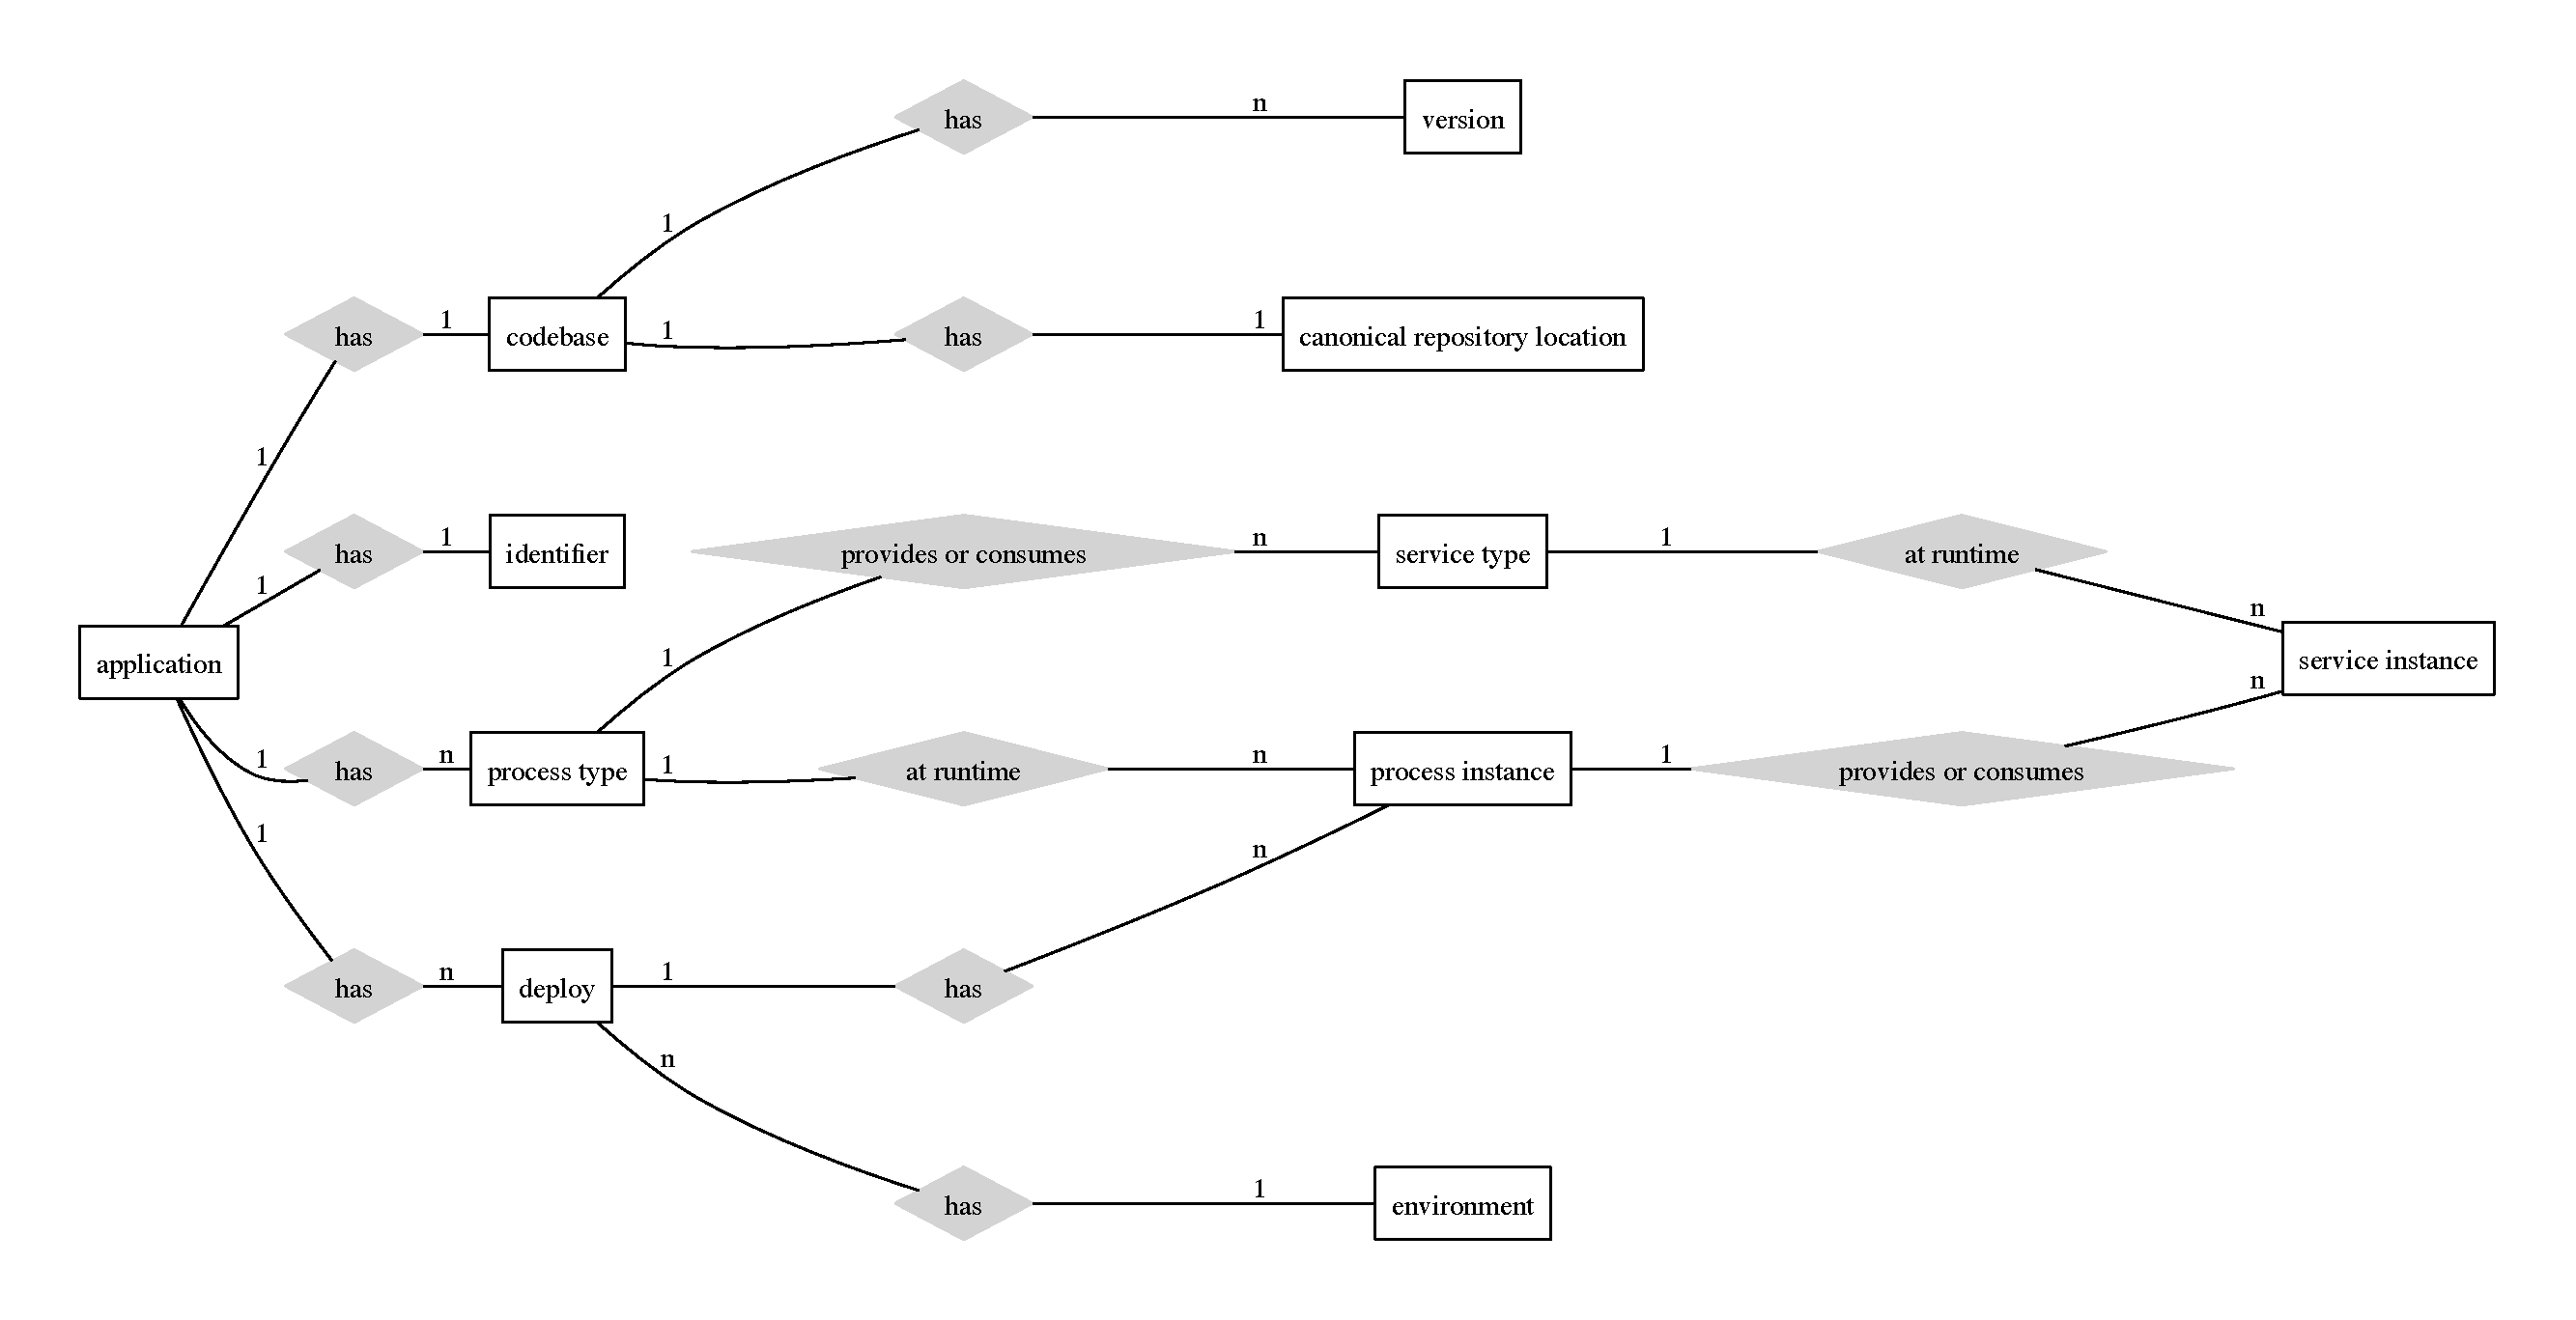
\includegraphics[width=1.15\linewidth] {images/env.pdf}}
\end{figure}

An \emph{application} is the implementation of capabilities. Capabilities manifest themselves as having a real-world effect \cite{modServicesAnalysis}. Usually the users of an application are able to observe its real-world effects during operation.

The following technical descriptions of \emph{applications} are related to the observations made by Wiggins~\cite{12factor} as part of ``12 factor applications'', but have been customized by us as core part of the terminology model, especially regarding the interrelation to other concepts. We visualize the interrelation of the described concepts in \autoref{fig:software-env-erm}.

Every application has exactly one \emph{codebase}. The codebase may consist of files that are required to execute the application (e.g. source code) as well as meta data (e.g. documentation). The codebase is tracked in a source code version control system like Git~\cite{ProGit} or Subversion~\cite{svn}. We assume that within that system there is a canonical location for the codebase repository. Within that repository, the codebase might exist in different versions. We assume that for every repository, there is always a canonical version that represents the current state of development.

When an application is executed at runtime, its concrete representation are \emph{processes}. One application may have many process types, each of which may have many process instances at runtime. We explain processes further below.

Every application has at least one identifier, which is unique in the current scope of investigation, which in our cases here is the organizational boundary of the company.
% We follow the definition in \cite{rfc3986}: ``An identifier embodies the information required to distinguish what is being identified from all other things within its scope of identification.". How the identifier is actually structured is less important for our works, but possibilities would be the ``Uniform Resource Identifier'' from \cite{rfc3986} or following the structure of the ``host'' component as defined in the same document.

We distinguish between \emph{internal} and \emph{external} applications, based on the boundaries of an organization. The development of an \emph{internal} application is driven within the organization. The development of an \emph{external} application is driven externally to the organization. We assume both application types to be executed within the organization, thus on the machines under the control of the organization. An \emph{external} application may also be executed outside of the organization if specified (e.g. services provided by other SaaS platforms).

Another categorization of applications we propose is between \emph{client-facing} and \emph{infrastructure} applications:
\begin{tdescription}
  \item[Client-facing applications] serve a \emph{client-facing} functionality. Thus, if such an application would be removed, the clients (and the human users of these) would notice a lack of functionality. Often these applications are very specific to the business they support.
  \item[Infrastructure applications] support the \emph{client-facing} applications in their operation, but in themselves do not provide a client-facing functionality. Thus, if the infrastructure application would be removed, the clients (or human users of these) would not notice a lack of functionality (given that the \emph{client-facing} applications were still able to operate). We will discuss infrastructure applications further in the following \nref{subsec:infrastructure}.
\end{tdescription}

In our work, we focus on \emph{client-facing} applications. Forth going when we talk about ``applications'', we implicitly exclude \emph{infrastructure} applications.

An application may have many \emph{deploys}, as explained next.

\subsubsection{Deploy}

A \emph{deploy} of an application consists of the application's process instances executed in a specific environment. It may also be referred to as an application at runtime. But since an application itself is an abstract entity, the concrete representation of it at runtime are its processes instances.

Every deploy is executed within a specific environment. Common names for such environments are ``production'' or ``staging''. For each environment, a deploy might be configured differently, for example with regards to runtime parameters like queue lengths and timeout thresholds, or the location of services to consume.

The deployment of an application is often facilitated by deployment systems, which we introduce later in \nref{subsec:deploymentsys}.

\subsubsection{Process}

A \emph{process} is the concrete representations of an application at runtime. One process always belongs to one application. One application may have many processes. A process may be seen from two viewpoints: as process instance and as process type.

A \emph{process instance} exists during execution, where it might use resources like CPU time, memory, files or I/O devices. The implementation details of how a process instance is managed during runtime is not of interest for our work, but we assume that its resources and lifecycle are managed by an operating system, for example as described by Silberschatz et al \cite{silberschatz1998operating}.

A \emph{process type} is a logical entity embodying the opportunity to execute process instances of it. A process type usually manifests itself in some way in the source code of an application, for example by being a dedicated software module.

Every process instance always has exactly one process type and one deploy, whereas a process type may have many process instances, which in may even belong to different deploys. When we speak of ``a process'' it embodies both concepts of \emph{process instance} and \emph{process type}, which may be used interchangeably depending on the current context of discussion.

A process may consume and provide many services, as explained next.

% An application might implement services, which might then be consumed by other applications. Vice versa it might also consume services, provided by other applications. If an application does neither provide nor consume a service, then it is not interesting in the investigations of this work.

\subsubsection{Service}

A \emph{service} provides access to the capabilities of an application to other applications via a network. The possible ways of access are defined through a service interface. A service interface might be standardized in a machine-readable format like a WSDL definition~\cite{wsw3c}, or just be defined through the implementation itself.

Services are implemented as processes. Just as with processes, we may speak about service types and service instances. Since each service may be consumable via a network, a service also needs to be addressable. Therefore each service instance may have a URI, via which it may be consumed by other processes.

If a process exposes its functionality via a service interface, it provides a service. If a process starts a connection to a service, it consumes that service.

% Contrary to definitions of services in ``web services'' \cite{w3carch} \cite{w3cwsa} as well as ``SOA'' \cite{enterpriseSOA}, we do not assume that services have machine-readable service interface descriptions. We also do not

The access to services is facilitated as machine-to-machine interaction over a network, as described next.

\subsubsection{Service communication}

\emph{Service communication} happens between a service consumer and a service via a network connection, over which they may exchange messages.

We assume that service consumer and service are interoperable over an agreed protocol stack which should adhere to the standards set by the Internet protocol suite \cite{internetprotocol}.

We do not assume anything on the communication pattern. Examples might be request-response \cite{requestresponse} or publish-subscribe \cite{publishsubscribe}. The service provider is always the process that accepts the connection. The service consumer is the process that established the connection.

We do not assume anything on the locality of the service and the service consumer. They might be on the same physical machine, in different datacenters, or within different organizations.

% An application may implement many services. It is then called a service provider. It may also be called a server, following the definition in \cite{rfc2616}: `` An application program that accepts connections''.
%
% An application that consumes services is called a service consumer. It may also be called a client, following the definition in \cite{rfc2616}: ``A program that establishes connections''.

\subsubsection{Service dependency}
\label{subsec:service_depenedency}

A \emph{service dependency} is the fact that a process is the consumer of a service. The service dependency is always directed from service consumer to service provider.

Given that a service dependency exists, it may also be noted with the related applications (as either service dependency or application dependency).

Please note that a service dependency is not to be confused with a shared library dependency: Both concepts have in common that the dependency is to another software component. These components are often developed in a different organizational context than the program that depends on it. This manifests itself in decoupled software life cycles. The difference between both concepts is that a shared library dependency is executed in the same context as the program (e.g. the same process) and usually used via an in-memory function call. On the other hand, a service dependency is executed in another context (e.g. another process, machine or datacenter) and therefore the communication may not happen via in-memory function calls, but through mechanisms like remote procedure calls \cite{Birrell1984} or web services \cite{wsw3c}.

\subsubsection{Machines}

A \emph{machine} consists of a CPU, memory, permanent storage and an operating system. Every machines is connect to a network and may be addressable and accessible over it. A machine might be physical or virtual, but is always under the full control of the organization. A machine provides the execution context for processes and might be used by \emph{client-facing} and \emph{infrastructure} applications alike.

\subsection{Infrastructure systems}
\label{subsec:infrastructure}

When building a microservice architecture, certain types of systems are commonly used to support its realization. We call these \emph{infrastructure system}, since they form the infrastructure for developers to build \emph{client-facing} applications on. In this section we will describe three types of infrastructure systems: \emph{deployment}, \emph{service discovery} and \emph{telemetry} systems. We introduce their concepts here and will describe the concrete implementations we found for them in our case study in later \nref{chapter:case_study}.

\subsubsection{Deployment systems}

For an application to be actually used at runtime, it needs to be deployed. A deployment procedure usually starts with the application's codebase and ends with process instances running.

The foundation for each deployment system is that there are available computing resources under control of the organization. The deployment system then matches available resources with processes of application deploys and cares for starting the process instances. This might include building the application, distributing the build artifacts to the correct machines, setting up the runtime and configuration environment as well as starting and supervising the processes at runtime. This implies that the deployment system has knowledge about existing applications and about currently running process instances.

It is possible to execute a deployment procedure manually without utilizing a dedicated deployment system. Engineering experience has shown that it is desirable to automate deployment procedures as much as possible in order to increase development speed and lower potential for failure. Humble et al \cite{ContinuousDelivery} motivate and describe this subject in detail.

\subsubsection{Service discovery}

When a process wants to consume the service of a certain application or deploy, it has to know the service's location. Service discovery answers this question, mapping an application name (and possible more qualifying information like deployment environment or datacenter) to the location of the services. Listing \ref{list:sd_example} shows an example of such a mapping. Since a deploy might have many process and service instances, service discovery might return the locations of all of these. Since we assume all service communication to happen via the TCP/IP protocol stack, the eventual format of a service locations is always an IP address and a port number.

\begin{lstlisting}[language=json,numbers=none,caption=Example for a service discovery mapping from service discovery key to service locations with IP address and port number,label=list:sd_example,backgroundcolor=\color{white}]
"myapplication" -> [ "10.20.30.1:123", "10.20.30.2:321"]
\end{lstlisting}

% Difference in how changes are propagated:
%
% Might be pull: client has to pull from source of service discovery, what the current configuration is
%
% Might be push: once the service discovery configration changes, it pushes these changes to all to all clients
%
% Might be tiered: initial entry point is pulled (and might also only be done once then), but from there service discovery is done on each call by another entity. Cases are load balancer (must now how to reach load balancer, from there load balancer knows all backends) or via message bus (must know location of message bus, message bus distributes to all recipients).

\subsubsection{Telemetry}

Telemetry is defined in \cite{merriamwebstertelemetry} as ``the process of using special equipment to take measurements of something (such as pressure, speed, or temperature) and send them by radio to another place''. Telemetry systems are the basis for reasoning about the current state of the system, since they collect measurements and present them to engineers in a queryable format. Telemetry systems are also used for setting up alerting. Since in a microservice architecture process instances are by definition distributed over many machines, a dedicated telemetry system is needed for effectively providing engineers with the relevant information about the systems state.

\section{Summary}

In this chapter, we first introduced aspects of dependability theory based on the ``dependability tree'' by Laprie (visible in \autoref{fig:laprie}). We described the dependability threats \emph{fault}, \emph{error} and \emph{failure} and how these relate to each other. Based on the categorization of faults into \emph{internal} and \emph{external} faults, we mentioned the \emph{chain of dependability threats} as a model to understand propagation of failures between interdependent systems. As attributes to qualify dependability we described \emph{reliability} and \emph{availability}. Afterwards we introduced qualitative and quantitative \emph{fault trees} as ways to model dependability.

To describe the microservice architectural style further we proposed an own terminology model. At the core it defines what an \emph{application} is and how applications may depend on each other through services. The interrelation of the introduced terms can be seen in \autoref{fig:software-env-erm}. We ended the chapter by introducing infrastructure systems that support the realization of microservice architectures.